% Created 2024-01-20 Sat 17:09
% Intended LaTeX compiler: pdflatex
\documentclass[11pt,a4paper,final]{article}
\usepackage[a4paper, total={7in, 10in}]{geometry}
\usepackage{algorithm2e}
\usepackage{booktabs}
\usepackage{subcaption}
\usepackage{graphicx}
\usepackage{tikz}
\usepackage[utf8]{inputenc}
\usepackage[T1]{fontenc}
\usepackage{graphicx}
\usepackage{longtable}
\usepackage{wrapfig}
\usepackage{rotating}
\usepackage[normalem]{ulem}
\usepackage{amsmath}
\usepackage{amssymb}
\usepackage{capt-of}
\usepackage{hyperref}
\usepackage{xcolor}                         % Color time
\usepackage{listings}                       % Code in LaTeX
\usepackage{listings-rust}                  % Code in LaTeX
\usepackage{amsfonts}                       % Cool math fonts
\usepackage{tabularx}                       % Cool tables
\usepackage{multicol}                       % Add capability to make columns
\usepackage{hyperref}                       % Cool clean hyperlinks
\setlength\parindent{0pt}                   % No indent for paragraphs
\lstset{language=Rust, style=boxed}
\usetikzlibrary{arrows.meta}                % Arrows for tikz
\renewcommand*{\sectionautorefname}{Section}
\renewcommand*{\subsectionautorefname}{Section}
\renewcommand*{\subsubsectionautorefname}{Section}
\renewcommand*{\paragraphautorefname}{Section}
\renewcommand*{\algorithmautorefname}{Algorithm}
\newcommand{\Or}{\textbf{ or }}
\renewcommand*{\And}{\textbf{ and }}
\newcolumntype{L}[1]{>{\hsize=#1\hsize\raggedright\arraybackslash}X}%
\newcommand\mycommfont[1]{\footnotesize\ttfamily\textcolor{gray}{#1}}
\newcommand{\T}{\mathcal{T}}                % To make it clear the difference
\newcommand{\Tau}{T}                        % between Tau and T
\newcommand{\AC}{AC(u, d, v, \eta)}         % Set the parameters for AC once
\newcommand{\UC}{UC(u, d, v)}               % Set the parameters for UC once
\newcommand{\ACi}{AC(u_i, d_i, v_i, \eta_i)}% Set the parameters for AC once
\newcommand{\UCi}{UC(u_i, d_i, v_i)}        % Set the parameters for UC once
\newcommand{\Not}{\textbf{not }}            % Custom `not' operator
\newcommand{\visit}{(i, b, a, e, u, d, v, \eta, \xi)}
\newcommand{\I}{\mathbb{I}}                 % Set of visit tuples
\newcommand{\C}{\mathbb{C}}                 % Charger availability information
\newcommand{\U}{\mathcal{U}}                % Uniform distribution
\newcommand{\Sol}{\mathbb{S}}               % A shorthand for visit tuple
\newcommand{\M}{\mathbb{M}}                 % A shorthand for the metadata
\newcommand{\Hd}{\mathbb{H}}                % Set of discrete times
\newcommand{\Nu}{\mathcal{V}}               % Draw a nice Nu
\newcommand{\Iset}{I}                       % Set of visits 1-I
\newcommand{\Isetinit}{I_0}                 % Set of visits inital visits
\newcommand{\Isetfinal}{I_f}                % Set of visits final visits
\newcommand{\Bset}{B}                       % Set of visits 1-B
\newcommand{\Qset}{Q}                       % Set of visits 1-Q
\newcommand{\Jset}{J}                       % Set of visits 1-J
\newcommand{\Jsetq}{\mathbb{J}}             % Set of visits 1-J for queue active times
\newcommand{\Hset}{H}                       % Set of visits 1-H
\date{\today}
\title{Bus Charging Schedule Simulated Annealing with MILP Constraints}
\hypersetup{
 pdfauthor={},
 pdftitle={Bus Charging Schedule Simulated Annealing with MILP Constraints},
 pdfkeywords={},
 pdfsubject={},
 pdfcreator={Emacs 29.1 (Org mode 9.6.6)}, 
 pdflang={English}}
\begin{document}

\maketitle
\tableofcontents

\parskip 3mm                                % Set the vetical space between paragraphs
\let\ref\autoref                            % Redifine `\ref` as `\autoref` because lazy
\SetCommentSty{mycommfont}                  % Set the comment color

\section{Introduction}
\label{sec:introduction}
This document outlines a Simulated Annealing (SA) approach to the bus charging scheduling problem that utilizes Mixed
Integer Linear Programming (MILP) constraints to determine feasible charging schedules. The problem involves generating
an optimal charging schedule for a fleet of Battery Electric Buses (BEBs) based on a set of routes and a mix of fast and
slow chargers. The aim is to minimize both the consumption cost (amount of electricity used over a certain time) and the
demand cost (rate at which electricity is being used) while ensuring that the buses maintain sufficient charge to
complete their workday without delays.

The SA algorithm is introduced and constrained by a set of MILP constraints derived from the Position Allocation Problem
(PAP) to ensure the validity of proposed charging schedules. Objective functions describing consumption cost and demand
cost are used to minimize power consumption and total cost of using the BEBs.
\section{Problem Description}
\label{sec:problem-description}
This section introduces and defines the problem to be addressed by this work. A general description is given and
followed by a mathematical interpretation. The scope of this work will also be provided as well as a high level
introduction to the granular problems that will be addressed in order to achieve the proposed goal.

Consider a fleet of BEBs scheduled to perform a set of prescribed routes on a given day. Suppose that an individual BEB
from said fleet begins and completes an individual route at the same station from which it also receives its charge.
During each route, the BEB's State of Charge (SOC) depletes by a certain amount. The charge supplied during its visit
must be enough that it sustains the BEB's SOC at an appropriate level such that it may complete its route. The charge
may be supplied from any single charger given a set of chargers at the station. Each time the BEB arrives at the
station, let that be denoted as an ``arrival''. Once the BEB has awaited its predetermined time (whether it has received a
charge or not), and departs from the station, let that be denoted as a ``visit''. Generalizing this to all BEBs, each BEB
will have a set of prescribed routes from which their SOC is depleted by a certain amount. Once the route is completed,
the BEB arrives at the station to receive a charge that is sufficient to complete the next route. Each BEB may have
multiple visits to the station throughout their working day. This paper describes a method to optimize the assignment of
each visit to a charger given a schedule for a fleet of BEBs that follow the behavior described above.

Consider a fleet of \(n_B\) BEBs that collectively visit a station \(n_I\) times. At said station, let there exist a pool of
\(n_Q\) charging queues from which a visiting BEB may be assigned. The set of arrivals is denoted as \(\Iset = \{ 1, ...
n_I \} \subset \mathbb{Z}\). Each BEB is provided an identification number \(B = \{ 1, ..., n_B \}\). Each visit can be represented by the
tuple: \(\visit\), in which the elements within the tuple denote the visit index, \(i \in I\), BEB identification number, \(b_i
\in B\), arrival time to the station, \(a_i \in \mathbb{R}\), departure time from the station, \(e_i \in \mathbb{R}\), time to start charging, \(u_i \in
\mathbb{R}\), time to stop charging, \(d_i\), the charger queue for the BEB to be placed into, \(v_i \in Q\), the SOC, \(\eta_i \in \mathbb{R}\), and
the index of the next visit for the currently visiting BEB, \(\xi_i \in I\). Let the set of all visits be denoted as \(\I\).

For each visit, a BEB must be placed in a single queue, \(q \in \Qset\). The charger \(q\) is assumed to be either a fast
charger, slow charger, or no charger at all (denoted as a waiting queue). A BEB is only allowed to be assigned to one
queue per visit; however, there may be multiple BEBs charging simultaneously across different queues. The amount of time
the BEB is allowed to charge is dictated by the scheduled arrival time and required departure time, \([a_i, e_i]\).
Partial charging is allowed; however, the SOC may not exceed the BEB battery capacity. The battery dynamics in this work
is modeled as \uline{linear}, which remains accurate up to about an SOC of 80\% charge \cite{li-2016-batter-elect}.

Each BEB arrival, except for the last arrival for each BEB, has a paired ``route'' that the BEB must perform after the
visit. This route, as one would expect, causes the BEB to discharge by some certain amount. The estimation of the SOC
post route in it of itself poses a focus of research, not of which is of this work. Thus, a simplified model of
calculating an average discharge based on the time a BEB is on route is employed. For visit \(i\), the route is assumed to
occur after its departure. Let the discharge of the route for visit \(i\) be denoted as \(\Delta_i \in \mathbb{R}\). The charge supplied
while at the station is required to increase the SOC of each BEB visit to a minimum battery percentage, \(\nu_b \in B\). This
acts as a safety factor to ensure each route is completed.

The task of this paper shall be to define a method of scheduling the set of visits \(\I\) to fulfill the minimum charge
requirements over the time horizon \(T\) while minimizing the cost, which can be decomposed into the demand and
consumption cost. An objective function is utilized to measure the relative fitness of results and constraints are
employed to ensure validity of the prescribed schedule. Both the objective function and constraints are discussed in
further detail in the proceeding section.
\section{Optimization Problem}
\label{sec:optimization-problem}
This sections introduces the problem in the form of the objective function as well MILP constraints. The objective
function is required to allow comparisons between candidate solutions. In the context of this formulation, the objective
function is broken down into four major components: consumption cost, demand cost, assignment cost, as well as a penalty
for under-charging a bus. The constraints ensure that candidate solutions are in the feasible region. They are composed
of a series of equations defined by decision and input variables. Decision variables are those which may be manipulated,
and are chosen in an attempt to optimize the objective function. Input variables are predefined.

The input and decision variables are introduced in \ref{sec:input-variables} and \ref{sec:decision-variables}. The
objective function is introduced in \ref{sec:objective-function}. The constraints will then be introduced in
\ref{sec:constraints}.

\subsection{Variable Definitions}
\label{sec:parameter-definitions}
This section defines the input and decision variables used by the system. The input parameters are assumed to be fixed
prior to optimizing the system. The decision variables are the values that the SA algorithm has the freedom to
manipulate.

\subsubsection{Parameters}
\label{sec:input-variables}
This section introduces the parameters used in the SA algorithm. The variables to be introduced are summarized in
\ref{tab:variables}. \(\Delta_i\) is the amount energy required to complete the bus route after visit \(i\). Because there is no route
after the last visit, the power consumed after the final visit is zero. Let the set of final visits for all BEBs be
denoted as \(\Isetfinal\). \(\alpha_b\) is the initial SOC percentage of bus \(b\) at the beginning of the working day. Let
\(\Isetinit\) denote the set of initial visit indices for each BEB. Let \(\Xi_i \in B\) denote the identification number of the
BEB for visit \(i\). The initial SOC for bus \(\Xi_i\) can be represented as \(\eta_{i \in \Isetinit} = \alpha_{\Xi_i} \cdot \kappa_{\Xi_i}\) where
\(\kappa_{\Xi_i}\) is the battery capacity for bus \(\Xi_i\), \(\eta_{i \in \Isetinit}\) indicates the initial charge for bus \(b\). The rest
value for \(\eta_i\), \(i \not\in I\) are considered decision variables and will be further discussed in \ref{sec:decision-variables}.
The notation \(dt_h\) is used to denote the discrete time employed in calculating the demand cost. \(\epsilon_q\) is the cost for
assigning a charger to queue \(q\). \(\xi_i\) represents the next arrival index for bus \(b_i\). In other words, suppose the ID
of each BEB is recorded in order of arrival. Further suppose that recorded list is \(\xi = \{ 2,1,3,2 \}\), using a starting
index of 1, \(\xi_1 = 4\) as that is the next visit by bus 2, the same as the first visit index. The arrival and departure
times of bus visit \(i\) to the station are denoted as \(a_i\) and \(e_i\), respectively. Lastly, \(r_q\) represents the power
supplied from the charger in queue \(q\).

\begin{table}[htbp]
\caption{\label{tab:variables}Table of variables used in the paper.}
\centering
\begin{tabularx}{\textwidth}{L{0.3} L{1.2} L{0.3} L{1.2}}
\textbf{Variable} & \textbf{Description} & \textbf{Variable} & \textbf{Description}\\[0pt]
\hline
Constants &  & Constants & \\[0pt]
\(C\) & Penalty method gain factor & \(n_B\) & Number of buses in use\\[0pt]
\(H\) & Number of discrete steps, \(h\), in time horizon & \(n_I\) & Number of total visits\\[0pt]
\(J(u,d,v,\eta)\) & Objective function & \(n_K\) & Number of discrete steps in time horizon\\[0pt]
\(M\) & Total number of steps created by initial temperature, \(\Tau_0\), and cooling schedule & \(n_Q\) & Number of chargers\\[0pt]
\(\T\) & Time horizon &  & \\[0pt]
\hline
Input variables &  & Input Variables & \\[0pt]
\(\Delta_i\) & Discharge of visit over after visit \(i\) & \(\alpha_b\) & Initial charge percentage time for bus \(b\)\\[0pt]
\(\delta_i\) & Discharge rate for vehicle \(i\) per mile & \(\nu\) & Minimum charge percentage allowed for each visit \(i\)\\[0pt]
\(\epsilon_q\) & Cost of using charger \(q\) & \(\kappa_b\) & Battery capacity for bus \(b\)\\[0pt]
\(\rho_i\) & Route distance after visit \(i\) & \(\xi_i\) & The next index bus \(b\) will arrive\\[0pt]
\(a_i\) & Arrival time of visit \(i\) & \(\Xi_i\) & ID for bus visit \(i\)\\[0pt]
\(dt_h\) & Discrete time step \(dt_h = t_h - t_{h-1}\) & \(e_i\) & Time bus visit \(i\) must exit the station\\[0pt]
\(k\) & Local search iteration \(k\) & \(m\) & Minimum charge percentage allowed for each visit\\[0pt]
\(r_q\) & Charge rate of charger \(q\) &  & \\[0pt]
\hline
Direct Decision Variables &  & Direct Decision Variables & \\[0pt]
\(u_i\) & Time to start charging for visit \(i\) & \(d_i\) & Time to detach bus from charger for visit \(i\)\\[0pt]
\(\mu\) & \(Q \times N\) matrix of binary variables such that \(\mu_h^{v_i} = 1\) if \(u_i \le dt_h\), 0 otherwise & \(\theta\) & \(Q \times N\) matrix of binary variables such that \(\theta_h^{v_i} = 1\) if \(d_i \ge dt_h\), 0 otherwise\\[0pt]
\(v_i\) & Assigned queue for visit \(i\) &  & \\[0pt]
Indirect Decision Variables &  & Indirect Decision Variables & \\[0pt]
\(\eta_i\) & Charge for the bus at the beginning of visit \(i\) & \(\iota\) & \(Q \times N\) matrix of binary values such that \(\iota_h^{v_i} = 1\) if \(u_i \le dt_h \le d_i\), 0 otherwise\\[0pt]
\(\phi_i\) & Binary term to enable/disable charge penalty for visit \(i\) & \(\psi_{ij}\) & Tracks spatial overlap for visit pair \((i,j)\)\\[0pt]
\(\sigma_{ij}\) & Tracks temporal overlap for visit pair \((i,j)\) & \(d_i\) & Detach time from charger for visit \(i\)\\[0pt]
\(p_{dem}(t)\) & Demand cost & \(s_i\) & Amount of time spent on charger for visit \(i\) (service time)\\[0pt]
\hline
\end{tabularx}
\end{table}

\subsubsection{Decision Variables}
\label{sec:decision-variables}
Decision variables are the chosen by the optimizer. The variables will be broken into two sections: direct and indirect
decision variables. Direct decision variables that are direct are values that the system has direct control over and
indirect variables are those that are influenced by the direct.

\paragraph{Direct Decision Variables}
\label{sec:direct-decision-variables}
The first two variables are \(u_i\) and \(d_i \; \forall i \in \Iset\). They represent the initial and final charging times. These
values must remain within range of the arrival time and departure time for visit \(i\), \([a_i, e_i]\). A method of
determining if a discrete time step \(dt_h\) is within the charging time for visit \(i\). Let \(n_T\) be defined as the total
number of discrete steps taken over the time horizon, \(\mu\) and \(\theta\) are \(n_T \times n_Q\) matrices of binary decision variables,
\(\mu_h^{v_i}, \theta_h^{v_i} \in \{0, 1\}\). \(\theta_h^{v_i} = 1\) when \(u_i \le dt_h\), and \(\theta_h^{v_i} = 0\) otherwise. \(\mu_h^{v_i} = 1\)
when \(d_i \ge dt_h\) and \(\mu_h^{v_i} = 0\) otherwise. The last direct decision variable is the queue that bus visit \(i\) can
be placed in to charge, \(v_i \in \Qset\).

\paragraph{Indirect Decision Variables}
\label{sec:indirect-decision-variables}
Let the initial SOC for a visit be written as \(\eta_i\), where \(i \in \Iset \setminus \Iset_0\) and \(\Iset_0\) denotes the set of
initial visits for each BEB. Note that \(\Iset_0\) is excluded from the set of decision variables because each BEB is
assumed to have a known SOC at the beginning of the working day. The initial charge for visit \(i\) forms the foundation
from which the SOC is calculated for the BEB's next visit, \(\xi_i\). This propagation of the SOC is evaluated as shown in
\ref{eq:bat-chain}. The equation states that the charge for bus \(i\)'s next visit is equal to the initial charge for visit \(i\)
plus the charge added to it by charger \(v_i\) over duration \(s_i = d_i - u_i\) minus the discharge accumulated over route
\(i\).

\begin{equation}
\label{eq:bat-chain}
  \eta_{\xi_i} = \eta_i + r_{v_i}s_i - \Delta_i
\end{equation}

As described in the previous section, a method of determining whether a discrete time \(dt_h\) is within the range \([u_i,
d_i]\) is desired. A third variable \(\iota_h^{v_i}\) is introduced to indicate if the inequality \(u_i \le dt_h \le d_i\) is true or
not. Specifically it indicates if \(dt_h\) is within an active charging period for the charger \(v_i\) which will assist in
calculating the demand cost. That is, \(\iota_h^{v_i} \in \{0,1\} = 1\) when \(\mu_h^{v_i} = 1\) and \(\theta_h^{v_i} = 1\). This topic
will be covered in more depth in \ref{sec:objective-function}.

A penalty method is to be implemented in the objective function that is enabled when the \(\eta_i\) falls below a defined
threshold. Let the activating boolean decision variable be denoted as \(\phi_i \in \{0,1\}\). \(\sigma_{ij}\) and \(\psi_{ij}\) are used to
indicate whether a visit pair \((i, j)\) overlap the same space as show in \ref{fig:spacial-and-temporal-constr}. Formally,
\ref{eq:bus-spat-temp} describes the relationship that \(\sigma_{ij}\) and \(\psi_{ij}\) uphold. That is, for every visit, if the start
charge time of visit \(j\) is greater than the end charge time of visit \(i\), then \(\sigma_{ij}\) is active (\(\sigma_{ij} = 1\)).
Similarly, if the queue for visit \(j\) is in a queue that is in a queue of lesser index than visit \(i\), then \(\psi_{ij}\) is
active (\(\psi_{ij} = 1\)). These variables will be further elaborated on in \ref{sec:constraints}.

\begin{subequations}
\label{eq:bus-spat-temp}
\begin{equation}
  \sigma_{ij} =
  \begin{cases}
    1 & \text{if } u_i \ge d_j, \; i \ne j\\
    0 & \text{otherwise}
  \end{cases}
\end{equation}

\begin{equation}
  \psi_{ij} =
  \begin{cases}
    1 & \text{if } v_i \ge v_j,\; i \ne j\\
    0 & \text{otherwise}
  \end{cases}
\end{equation}
\end{subequations}

\(p_d\) is the demand cost of the overall charging schedule. It is calculated after all the decision variables have been
assigned. This is further described in \ref{sec:objective-function}.

\subsection{Objective Function}
\label{sec:objective-function}
The objective function is used to compare the fitness of different candidate solutions against one another. This
objective function takes in input and decision variables to calculate some value of measure. The calculated objective
function value can either be maximized or minimized. The desired option is dependent on the problem to be solved as well
as the formulation of said objective function. Let \(J\) represent the objective function. The objective function for this
problem has four main considerations: charger assignment, consumption cost, demand cost, and penalty on insufficient
charge. These considerations are divided into two components: The usage cost and the assignment cost.

Suppose the objective function is of the form \(\text{min } J = \AC + \UC\). \(\AC\) is the assignment cost, and \(\UC\) is
the usage cost. The assignment cost represents the costs of assigning a bus to a particular queue as well as the chosen
charging period, \([u_i, d_i]\). \(v_i \in \Qset\) is the charger index, \(u_i\) is the initial charge time, \(d_i\) is the detach
time for visit \(i\), \(\phi_i\) is a binary decision variable, \(m\) is the minimum charge percentage allowed, \(\kappa_i\) is the
battery capacity for visit \(i\), and \(\eta_i\) is the initial charge for visit \(i\).

\begin{equation}
\label{eq:ac}
\AC = \sum_{i=1}^I \Big(\epsilon_{v_i}r_{v_i} + \frac{1}{2} C \phi_i (\eta_i - m \kappa_i)^{2}\Big)
\end{equation}

The first term in the summation represents the calculation of the cost for assigning a bus to queue \(q\). Let \(\epsilon_{vi}\) to
be taken as \(\epsilon_{v_i} = 1000v_i\), this form encourages the objective function the minimize the total amount of chargers.
Iterating on this concept, let the model represents the first \(n_B\) indices to be waiting queues (no charge is
supplied), the next \(n_{Q_s}\) indices to be slow chargers, and the next \(n_{Q_f}\) indices to be fast chargers, where
\(n_B, n_{Q_s}, n_{Q_f} \in \mathcal{Z}\) and \(n_B + n_{Q_s} + n_{Q_f} = n_Q\). Furthermore, let \(\epsilon_b = \{ 0 : b \in \Bset \}\), \(\epsilon_{j} =
\{ 1000 j: j \in \Iset \}\) and let \(\epsilon = \epsilon_b \cup \epsilon_j\). That is, \(\epsilon_{v_i}\) has no cost if \(v_i \in \epsilon_b\) or is incrementally
penalized as the selected queue index increases if \(v_i \in \epsilon_j\). This form accrues no cost when assigning a BEB to a
waiting queue while still encouraging the use of slow chargers over fast.

The second term is the penalty function that is either enabled or disabled by \(\phi_i\)
\cite{luenberger-2008-penal-barrier-method}. The penalty function is enabled, \(\phi_i = 1\), if the SOC falls below a
specified SOC threshold, \(\eta_i \le \nu \kappa_{\Xi_i}\), and is disabled, \(\phi_i = 0\), otherwise. This term is considered an assignment
cost because the penalty method is enabled due to poor allocations of BEBs. That is, the cost is not impacted by how
much the system consumes energy, but by how the BEBs have been assigned. \(C\) is a large constant value used to scale the
penalty function. The mechanisms that enables or disables \(\phi_i\) is derived in \ref{sec:constraints}.

The usage cost is composed of the consumption cost and the demand cost. The consumption cost is merely the summation of
all the energy being used over all the active periods for each charger in the time horizon as written in
\ref{eq:consumption-cost}. \(r_{v_i}\) is the charge rate for the active charger \(v_i\) and is multiplied by the time that the
charger will be utilized, \(s_i\).

\begin{equation}
\label{eq:consumption-cost}
  \sum_{i=1}^I r_{v_i}s_i
\end{equation}

The demand cost quantifies the amount of power being used over a given period of time and increases the cost if too much
power is utilized within said period. A typical period in which to calculate the demand cost is over 15 minute
increments (0.25 hours). Let the average power used over an arbitrary 15-minute interval be represented by \ref{eq:p15}.

\begin{equation}
\label{eq:p15}
p_{15}(t) = 0.25 \int_{t-0.25}^{t} p(\tau) d\tau
\end{equation}

Worst case must be assumed to ensure enough power is available during peak hours; therefore, the maximum value found is
retained.

\begin{equation}
\label{eq:pmax}
p_{max}(t) = \max\limits_{\tau \in [0,t]}p_{15}(\tau)
\end{equation}

\ref{eq:pmax} is thus a function that describes the largest demand cost found up to time \(t\). A fixed minimum average power is
introduced that is intended to act as a base threshold before the cost begins to increase. Let this fixed threshold be
defined as \(p_{fix}\). Furthermore, let \(z\) define the demand rate which has the units of \(\frac{\$}{kW}\).

\begin{equation}
\label{eq:pdem}
p_d(t) = \max(p_{fix},p_{max}(t))z
\end{equation}

\ref{eq:pdem} then begins with a value of \(p_{fix}\) from which only increases if \(p_{15}(t) > p_{fix}\). To write the total
demand at any discrete time, consider \ref{eq:discrete-power}. Let \(\omega_h \in \omega\) be the discrete power demand at time step \(h\)
where \(h \in \{ 1, 2, ..., n_T \} \subset \mathcal{Z}\), \(n_T = \frac{T}{0.25}\), and \(\omega\) is an \(n_T \times 1\) vector. For conciseness of
notation we will abuse \(t_h\) to denote the time in discrete form (as opposed to \(t\) being continuous), let \(dt_h = t_h -
t_{h-1}\), and \(\Hset = \{ 1, 2, ..., n_T \}\). Let \(\iota\) be a \(n_T \times n_Q\) matrix of binary variables that is enabled if
charger \(v_i \in \Qset\) is active during the time frame \(dt_h\) and \(r\) is a \(n_Q \times 1\) vector of charger rates. Thus, the
discrete power utilized over the time horizon is calculated as follows.

\begin{equation}
\label{eq:discrete-power}
  \omega = \iota r
\end{equation}

Let \(M = 0.25/dt_h\) express the number discrete steps that spans a 15-minute interval. The average power over an
arbitrary 15-minute interval in the time horizon can be written as

\begin{equation}
p_{15}[h] = \sum_{h-M+1}^h \omega_h,
\end{equation}

where \(h \ge M\). Similarly to before, the maximum \(p_{15}[h]\) value is to be retained via \(p_{max} = \max\limits_{h \in
H}p_{15}[h]\). Thus, the discrete demand cost is expressed as shown in \ref{eq:pd-dis}.

\begin{equation}
\label{eq:pd-dis}
  p_d = \max(p_{fix}, p_{max})z
\end{equation}

To write the usage cost, \ref{eq:consumption-cost} and \ref{eq:pd-dis} are added together to create \ref{eq:pc}.

\begin{equation}
\label{eq:pc}
\UC = p_d + \sum_{i=1}^I \Big( r_{v_i}s_i \Big)
\end{equation}

\subsection{Constraints}
\label{sec:constraints}
Now that a method of calculating the fitness of a schedule has been established, a method for determining the
feasibility of a schedule must be defined. The feasible space for schedules defines the space in which the supplied
input and decision variables describe a schedule that would keep the BEBs adequately charged throughout the working day.
To ensure the selected decision variables fall within the feasible space, a set of constraints are applied to a given
candidate solution. The constraints must ensure no overlap temporally or spatially, receives enough charge to complete
its next route, the BEB cannot be over-charged, and the BEB must depart on time. The aforementioned constraints are
shown in \ref{eq:constraints}.

\begin{multicols}{2}
\begin{subequations}
\label{eq:constraints}

  \begin{equation}
      \label{seq:c0}
      u_i - d_j - (\sigma_{ij} - 1)T \ge 0
  \end{equation}
  \begin{equation}
      \label{seq:c1}
      v_i - v_j - 1 - (\psi_{ij} - 1)Q \ge 0
  \end{equation}
  \begin{equation}
      \label{seq:c2}
      \sigma_{ij} + \sigma_{ji} \le 1
  \end{equation}
  \begin{equation}
     \label{seq:c3}
      \psi_{ij} + \psi_{ji} \le 1
  \end{equation}
  \begin{equation}
      \label{seq:c4}
      \sigma_{ij} + \sigma_{ji} + \psi_{ij} + \psi_{ji} \ge 1
  \end{equation}
  \begin{equation}
      \label{seq:c5}
      s_i = d_i - u_i
  \end{equation}
  \begin{equation}
      \label{seq:c6}
       \eta_{\xi_i} = \eta_{i} + r_{v_i}s_i - \Delta_i
  \end{equation}
  \begin{equation}
      \label{seq:c7}
      \kappa_{\Xi_i} \geq \eta_{i} + r_{v_i}s_i
  \end{equation}
  \begin{equation}
      \label{seq:c8}
      \eta_{i} + r_{v_i}s_i - \Delta_i \ge \nu \kappa_{\Xi_i}
  \end{equation}
  \begin{equation}
      \label{seq:c9}
      \eta_{i} - m\kappa_{b_i} \le T (1 - \phi_{i})
  \end{equation}
  \begin{equation}
      \label{seq:c10}
      m_{k_i} - \eta_{i} > T \phi_{i}
  \end{equation}
  \begin{equation}
      \label{seq:c11}
      a_i \leq u_i \leq d_i \le e_i \le T
  \end{equation}
  \begin{equation}
      \label{seq:c12}
      dt_h - u_i \le T\theta_h^{v_i}
  \end{equation}
  \begin{equation}
      \label{seq:c13}
       u_i - dt_h \le T(1 - \theta_h^{v_i})
  \end{equation}
  \begin{equation}
      \label{seq:c14}
      d_i - dt_h \le T\mu_h^{v_i}
  \end{equation}
  \begin{equation}
      \label{seq:c15}
      dt_h - d_i \le T(1 - \mu_h^{v_i})
  \end{equation}
  \begin{equation}
      \label{seq:c16}
      \iota = \mu \circ \theta
  \end{equation}
\end{subequations}
\end{multicols}

Constraints \ref{seq:c0}-\ref{seq:c4} are the ``queuing constraints''. They are preventing overlap both spatially and
temporally as shown in \ref{fig:spacial-and-temporal-constr}. The y-axis represents the possible queues for a bus visit to be
placed into, and the x-axis represents the time that can be reserved for each visit. The shaded rectangles represent
time that has been scheduled in the x-axis, and the queue allocated for each bus visit in the y-direction. In other
words, the set of constraints \ref{seq:c0} - \ref{seq:c4} aim to ensure that these shaded rectangles never overlap.

\begin{figure}[ht!]
  \centering
  \scalebox{0.5}{
  \centerline{
    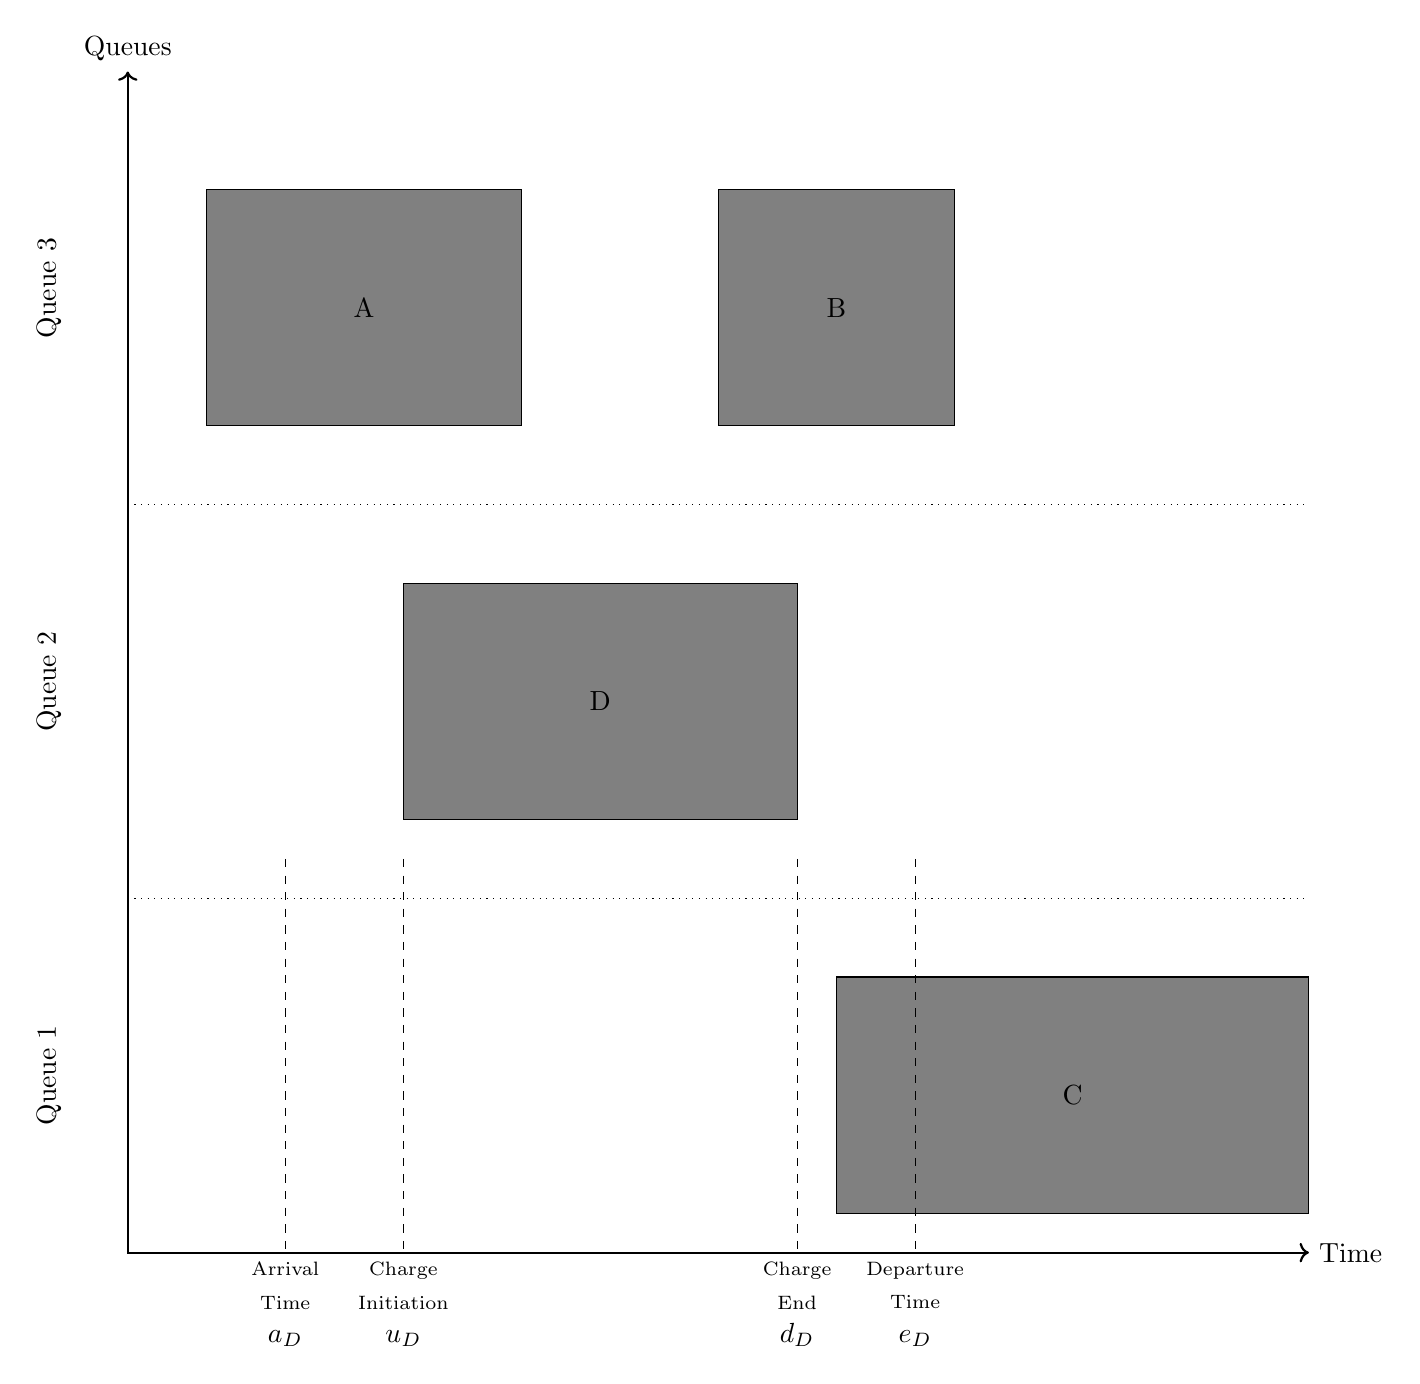
\begin{tikzpicture}
      % Variables
      \def \arrx   {2.0}
      \def \initx  {3.5}
      \def \endx   {8.5}
      \def \depx   {10.0}
      \def \yshift {5}

      % Axis
      \draw [thick,<->] (0,15) node[above]{Queues} -- (0,0) -- (15,0) node[right]{Time};

      % Rectangles
      \node[rectangle, draw, fill=gray, minimum width=4cm, minimum height = 3cm] at (3,12) {A};
      \node[rectangle, draw, fill=gray, minimum width=3cm, minimum height = 3cm] at (9,12) {B};
      \node[rectangle, draw, fill=gray, minimum width=5cm, minimum height = 3cm] at (6,7) {D};
      \node[rectangle, draw, fill=gray, minimum width=6cm, minimum height = 3cm] at (12,2) {C};

      % X-axis labels
      \node [below,align=center] at (\arrx,0) {\scriptsize Arrival     \\ \scriptsize Time \\ $a_D$};
      \node [below, align=center] at (\initx,0) {\scriptsize Charge    \\ \scriptsize Initiation  \\ $u_D$};
      \node [below, align=center] at (\endx,0) {\scriptsize Charge     \\ \scriptsize End \\ $d_D$};
      \node [below, align=center] at (\depx,0) {\scriptsize Departure  \\ \scriptsize Time \\ $e_D$};

      % Y-axis labels
      \node[rotate=90] at (-1, 2.25) {Queue 1};
      \node[rotate=90] at (-1, 7.25) {Queue 2};
      \node[rotate=90] at (-1, 12.25) {Queue 3};

      % Vertical lines
      \draw[dashed] (\arrx,\yshift)--(\arrx,0);
      \draw[dashed] (\initx,\yshift)--(\initx,0);
      \draw[dashed] (\endx,\yshift)--(\endx,0);
      \draw[dashed] (\depx,\yshift)--(\depx,0);

      % Horizontal lines
      \draw[dotted] (0, 4.5) -- (15, 4.5);
      \draw[dotted] (0, 9.5) -- (15, 9.5);

    \end{tikzpicture}
  }}
  \caption{The representation of the berth-time space. The x and y-axis represent time and space, respectively. Along the y-axis, the dashed lines represent discrete berthing locations. These locations may be chosen to be continuous. The shaded rectangles represent schedules vessels to serviced. The height of each shaded rectangle represents the space taken on the berth and the width being the time to service said vessel. The vertical dasched lines are associated with vessel D and represent the arrival time, berthing time, sercivce completion time, and departure time. Note that the arrival time may be before the berthing time and the completion time may before the departure time.}
  \label{fig:spacial-and-temporal-constr}
\end{figure}

Constraint \ref{seq:c4} states that the starting service time for BEB \(i\), \(u_i\), must begin after the previous BEB
departs, \(d_j\). The last term utilizes big-M notation to activate or deactivate the constraint. A value of \(\sigma_{ij} = 1\)
will activate the constraint to ensure that bus \(j\) is complete before bus \(i\) is allowed to begin being serviced. If
\(\sigma_{ij} = 0\), then the constraint is of the form \(T + d_j > u_i\) rendering the constraint ``inactive'' because \(u_i\)
cannot be larger than \(d_i\). This effectively allows the charging windows of the vehicle to overlap.

Similarly, \(\psi_{ij}\) determines whether the vehicles will be charging in the same queue. If \(\psi_{ij} = 1\) then
\eqref{seq:c1} is active; thus, vehicle \(j\) is in a queue index that is less than BEB \(i\). If \(\psi_{ij} = 0\) then the
constraint is deactivated and BEB \(j\) is in a queue index greater than that of BEB \(i\).

\ref{seq:c5} describes the service time of the bus. \ref{seq:c6} calculates the initial charge for the next visit for
bus \(b_i\). \ref{seq:c7} ensures that the bus is not being over-charged. \ref{seq:c8} ensures that the BEB's SOC does not
go below 0. \ref{seq:c9} and \ref{seq:c10} are used to enable and disable the penalty method in \ref{eq:ac}. This is done by
checking if the initial charge for visit \(i\) is greater than or equal to the minimum allowed charge. \ref{seq:c11}
ensures the continuity of the times (i.e. the arrival time is less than the initial charge which is less than the detach
time which is less than the time the bus exits the station and all must be less than the time horizon).

The last set of constraints \ref{seq:c12} - \ref{seq:c16} specifies the rule set for the decision variable \(\iota\). These
constraints define three \(n_T \times n_Q\) matrices that enforce \(\iota_h^q = 1\) if \(q = v_i\) and \(u_i \le dt_h \le d_i\), \(\iota_h^q = 0\)
otherwise. \ref{seq:c12} and \ref{seq:c13} utilizes big-M notation to ensure that the initial charge time for visit \(i\),
\(u_i\), is greater than or equal to the discrete time, \(0.25 \cdot h\). That is, \(\mu_h^{v_i} = 1\) if \(u_i dt_h\), \(u_h^{v_i} =
0\) otherwise. Similarly, \ref{seq:c14} and \ref{seq:c15} ensures that the final charge time, \(d_i\), is less than or
equal to the next discrete time step, \(dt_h\). The final constraint \ref{seq:c16} is a \(n_T \times n_Q\) matrix that represents
whether charger \(v_i \in \Qset\) is active. Note that \(\circ\) represents the Hadamard Product \cite{horn-1985-matrix-analy}.
Let \(A\) and \(B\) be two \(n_M \times n_N\) matrices. The Hadamard Product is defined as the element-wise product of the two
matrices, \(A \circ B = [a_{ij}b_{ij}]\).
\section{Simulated Annealing}
\label{sec:simulated-annealing}
SA is a well-studied local search metaheuristic used to solve discrete and (to a lesser degree) continuous problem
\cite{gendreau-2018-handb-metah}. A metaheuristic is a high-level problem-independent algorithm framework that provides
a set of guidelines or strategies to develop heuristic optimization algorithms \cite{radosavljevic-2018-metah-optim}.
Metaheuristic problems primarily fit in two categories: population-based and single-solution-based. Population based
algorithms emphasize exploration of the solution space as apposed to single-solutions-based algorithms being more
exploitation oriented \cite{radosavljevic-2018-metah-optim}. Generally, metaheuristic algorithms share the basic
advantage of speed in finding a satisfactory solution for large-scale practical optimization problems
\cite{radosavljevic-2018-metah-optim}. SA, however, is sometimes criticized for the speed at which it converges to the
global optimum \cite{gendreau-2018-handb-metah,henderson-1989-theor-pract}.

SA is an exploitation oriented, single-solution based metaheuristic with, in addition the previously stated, advantages
of simplicity, both theoretically and implementation, as well as its inherit ability to overcome non-linearities
\cite{gendreau-2018-handb-metah,radosavljevic-2018-metah-optim}. This model is named after its analogized process
where a crystalline solid is heated then allowed to cool at a slow rate until it achieves its most regular possible
crystal lattice configuration \cite{henderson-1989-theor-pract}. SA establishes a connection between this thermodynamic
and searching for global optima for an optimization problem.

There are five key components to SA: initial temperature, cooling schedule (temperature function), generation
mechanisms, acceptance criteria, local search iteration count (temperature change counter)
\cite{keller-2019-multi-objec}. The temperature solution describes the speed at which the system is ``cooled'' over each
iteration. The temperature of the system describes the likelihood that a system is willing to explore the solution
space. The generation mechanisms provide a means of modifying the system by some singular discrete change. The
acceptance criteria is a function of the system temperature that makes the decision whether the system will accept an
inferior solution in favor of exploring the solution space. Finally, the local search iteration count is the number of
steps taken to try to exploit a solution at a constant temperature. Each of these mechanisms are elaborated in the
subsequent sections.

\subsection{Cooling Equation}
\label{cooling-equation-experimental}
The temperature function models a ``rate of cooling'' for the SA process. Initially, when the temperature is high, SA
encourages exploration. As the process begins to ``cools down'' (in accordance to the cooling schedule), it begins to
encourage local exploitation of the solution (rather than exploration)
\cite{rutenbar-1989-simul-anneal-algor,henderson-1989-theor-pract}. There are three common basic types of cooling
equations: linear, geometric, and exponential. Each schedule is depicted in \ref{fig:cool} \cite{keller-2019-multi-objec}.
Each plot begin with an initial temperature of \(500^\circ\; C\) and a final temperature of \(1^\circ\; C\). The different cooling
schedules dictate the rate at which the algorithm progressively disallows exploration. A linear cooling schedule is
defined by \ref{eq:cool0}.

\begin{equation}
\label{eq:cool0}
\Tau[n] = \Tau[n-1] - \Delta_0
\end{equation}

with \(\Tau[0] = \Tau_0\) and \(\Delta_0 = 1/2\; C^\circ\) in \ref{fig:cool}. The value of \(\Delta_0 \in \mathbb{R}^+\). A geometric cooling schedules is as
defined in \ref{eq:cool1}. The cooling schedule type most widely used in practice \cite{keller-2019-multi-objec}. As such, it
will also be employed by the work in this paper.

\begin{equation}
\label{eq:cool1}
\Tau[n] = \alpha \Tau[n-1]
\end{equation}

where \(\alpha = 0.995\) in \ref{fig:cool}. \(\alpha\) may vary anywhere between the range \([0,1)\). An Exponential cooling schedule is
defined by the difference equation is defined as \ref{eq:cool2}.

\begin{equation}
\label{eq:cool2}
\Tau[n] = e^{-\beta}\Tau[n-1]
\end{equation}

where \(\beta = 0.01\) in \ref{fig:cool}. A typical range for \(\beta\) is \(0.8 \le \beta \le 0.99\) \cite{delahaye-2019-simul}.

\begin{figure}[htbp]
\centering
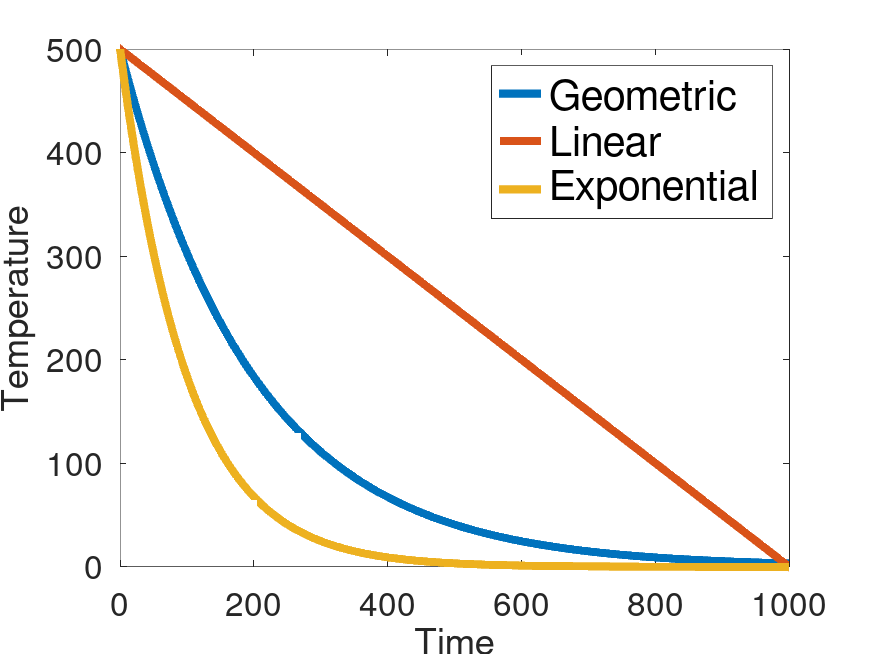
\includegraphics[width=0.5\textwidth]{sections/img/cool_func.png}
\caption{\label{fig:cool}Cooling equations}
\end{figure}

\subsection{Acceptance Criteria}
\label{sec:acceptance}
In SA, the algorithm stores a candidate solution that is continuously compared to newly generated solutions. Let the
stored solution be referred to as the ``active solution''. During each iteration, a new candidate solution is generated
and compared to the active solution to determine if the new solution should replace the active solution. In order to
determine if the active solution is to be replaced, an acceptance criteria is defined. A new candidate solution that is
more fit than active solution (fitness being dictated by the objective function) is always accepted as the new active
solution. In an effort to encourage exploration, inferior candidate solutions have a probability of being accepted as
the active solution. The probability of accepting an inferior candidate solution is described by the function
\(\exp(-\frac{J(x) - J(x')}{\Tau})\) where \(J(\cdot)\) is the objective functions described in \ref{sec:objective-function} and
\(\Tau\) is current temperature. The probability of acceptance is a function of the current temperature and the difference
of the active solution and a new candidate solution. Formally, let \(\Delta E \equiv J(x) - J(x')\) where \(x\) is the current
solution and \(x'\) is the new candidate solution. Let \(f(\cdot)\) be the function that describes the probability of accepting
a candidate solution \(x'\), and is defined by \ref{eq:candaccept} \cite{keller-2019-multi-objec}.

\begin{equation}
\label{eq:candaccept}
f(x,x',T) =
\begin{cases}
  1                   & \Delta E > 0 \\
  e^{- \frac{\Delta E}{T}} & \text{otherwise}
\end{cases}
\end{equation}

\subsection{Generation Mechanisms}
\label{sec:generation-mechanisms}
Generation mechanisms are used to create a neighboring candidate solution. That is, the generating function creates a
solution that can be reached in a single iteration from the active solution. In the case of the problem statement made
in \ref{sec:problem-description}, six primitive generation mechanism shall be used: new visit, slide visit, new charger,
wait, new window, and purge. The purpose of each of these generators is to assign new visits to a charger, adjust a bus
visits initial and final charge time within the same time frame/queue, move a BEB from one charger to another with the
same charge schedule, move a bus to its waiting queue, and remove a charger from the set of charger availability's. Each
generator will be discussed in more detail in \ref{sec:generators}.

These generator mechanisms will in turn be utilized by two wrapper functions. The schedule generation is to used create
candidate solutions for SA to compare with other solutions, and the perturb schedule generator is used to take a
candidate solution and alter it slightly in an attempt to fall into a global/local minimum. The wrapper functions will
be discussed in \ref{sec:generator-wrappers}. However, prior to discussing the primitives and wrapper generating functions,
their respective inputs and outputs must be defined.

\subsubsection{Generator Input/Output}
\label{sec:generator-input-output}
This section discusses in detail the expected inputs and output of each generator. It is important to discuss these
parameters to have an understanding of the generator algorithms to be derived. The input consists of the bus visit index
of interest, information about the current state of visits, \(\I\), and the current state of the charger availability,
\(\C\). The availability of each charger, \(\C\), is iteratively constructed during the SA process. The output of each
generator affects the tuple of decision variables \((v_i, u_i, d_i)\) and charger availability \(\C\).

\paragraph{Generator Input}
\label{sec:org90812c5}
Each generator an input of the tuple \(\Sol \equiv (i, \I, \C)\) where \(i\) is the visit index being manipulated, \(\I\) is the
tuple \(\visit\) as shown in \ref{sec:problem-description}, that describes the set of visits, and \(\C\) is the set that
describes the availability for all chargers \(q \in \Qset\). In other words, \(\C\) defines the set of times when the chargers
are not being utilized or are ``inactive''.

To derive \(\C\), consider its complement, \(\C'\), which is the set of ``active'' time periods for each charger. Let \(\C_q' \subset
\C'\) describes the active times for charger \(q\). Focusing on an individual charger, consider \(\C_q'\) before a schedule
has been imposed upon it, \(\C_q' = \{ \varnothing \}\). In other words, no buses have been assigned to be charged over
some time period \([u_i, d_i]\). After the scheduling process is complete, \(\C_q'\) will have a set of active periods of
the form \(\C_q' = \{[u_j, d_j]: j \in \Jsetq \}\) where \(\Jsetq \subset \mathcal{I}\). With a fully defined set \(\C_q'\), its compliment can
be found, \(\C_q\).

Let \(j\text{th}\) inactive period shall be denoted as \(\C^j_q\). To determine the inverse of \(\C_q'\), begin by noting
\(\C_q' \bigcap \{[u_j, d_j] : j \in \Jsetq\} = \varnothing\), is said to be disjoint (i.e. the sets share no common elements)
\cite{halmos-1974-naive-set-theor}. The inverse of a disjoint set can be found by the De Morgan Law: \((A \cap B)' = A' \cup
B'\). Using De Morgan's Law, the set of inactive periods can be written as \(\C_q \equiv \bigcup \{[u_j, d_j]': j \in \Jsetq\}\).

\paragraph{Generator Output}
\label{sec:orgba804e8}
The output of the generating functions is a modified subset of an input tuple. Let a modified input tuple be denoted as
\(\bar{\Sol}\) and the modified subset of the tuple be defined by \(\bar{x}_i \equiv (v_i, u_i, d_i, \C') \subset \Sol\), (as opposed
to \(x_i\) being unmodified). To be explicit, \(\bar{x}_i\) consists of the modified charger inactive times and the direct
decision variables: the chosen queue, initial charge time, and detach time from the charger. The other direct variables
and indirect variables may be implied. As previously discussed, early on in the SA process, the algorithm attempts to
encourage exploration by allowing candidate solutions of lesser quality be the active solution. To explore the feasible
space, the generators are employed with a sense of randomness to their respective outputs. Because of that, the modified
subset of the tuple, \(\bar{x}_i\), may be considered a random variable. Let the set of states for the output be defined
as \(\bar{x}_i \in \bar{x}_i \subset \bar{\Sol}\) where \(\bar{x}_i\) defines the feasible region for the subset of decision
variables.

\subsubsection{Generators}
\label{sec:generators}
This section describes and outlines the algorithm pool for the different generator types that are utilized in the
wrapper functions. Note that to satisfy constraints, \(n_B\) extra idle queues are added that provide no power to the bus.
Because of this, the set of queues is fully defined as \(q \in \{1,..., n_B, n_B+1,..., n_Q+n_B\}\) where \(n_Q\) is the total
amount of chargers and \(n_B\) number of BEBs. The use case for the idle queues are for when a bus is not to be placed on
a charger. Rather, it will be placed in the queue, \(v_i \in \{1,..., n_B\}\), which satisfies the previously defined
spatial constraints while allowing the bus to be ``set aside''.

In the development of the algorithms, dot notation is to be introduced to extract variables from tuples. For example,
suppose the arrival time is desired to be extracted from visit \(i\). Given \(\S\), the notation that describes extracting
\(u_i \equiv \I_{i.u}\).

\paragraph{New visit}
\label{sec:new-visit}
The new visit generator describes the process of moving an unsigned BEB \(b\) to a charging queue, \(v_i \in \{n_B+1,...,
n_B + n_Q\}\) within its arrival/departure time \([a_i, e_i]\). Let \(\U_{\cdot}\) indicate that an element is selected randomly
with a uniform distribution from the set \(\{\cdot\}\). For example, \(\U_{[a_i, e_i]}\) indicates that a value will be selected
between \(a_i\) and \(u_i\) with a uniform distribution. Lines 2 and 3 of \ref{alg:new-visit} extract the arrival and
departure times of visit \(i\). Note that in subsequent algorithms these lines will be omitted for conciseness. Lines 4
and 5 select a charging queue, \(q\), and time slice for which \(q\) is available at random with uniform distributions,
respectively. Line 6 quickly verifies that the inactive period selected is a viable selection and returns a random
charging time, \([u_i, d_i]\). If the time frames of the visit and the charger availability do not align, a tuple of null
values is returned.

The function \texttt{findFreeTime} is the algorithm that determines whether a visit's time at the station \([u_i, e_i]\) can be
placed in the time availability of charger \(q\). The algorithm is defined in \ref{alg:find-free-time}. Let \(L\) and \(U\) be
the lower and upper bound of the time between scheduled times. The set of cases is shown in \ref{fig:find-free}. In each case
depicted by \ref{fig:find-free}, the red line shows the arrival and departure time for a BEB visit, \(i\). The blue lines
indicate regions in which charger \(v_i\) is active. \(C \in \C_q \subset \C\) represents one of the ranges between the blue lines,
\([L, U]\), which stand for the lower and upper bounds of the region, respectively. That is, the only scheduling
constraint is that the arrival time is before charger \(q\) is available to charge the bus. Therefore, the bus must wait
until \(L\) before changer \(q\) may charge it. Furthermore, the range that \(u_i\) must be selected from is \([L,e]\). Lines
24-26 update the times slices for which charger \(q\) is available.

\begin{algorithm}[H]
  \caption{New visit algorithm} \label{alg:new-visit}
  \LinesNumbered
  \TitleOfAlgo{New Visit}
  \KwIn{($\Sol$)}
  \KwOut{$\bar{\Sol}$}

  \SetKwFunction{Union}{Union}
  \SetKwFunction{findFreeTime}{findFreeTime}

  \Begin {
    $a_i \leftarrow \I_{i.e}$\tcc*{Extract the arrivial time for visit $i$}
    $e_i \leftarrow \I_{i.e}$\tcc*{Extract the departure time for visit $i$}
    $q \leftarrow \mathcal{U}_{Q}$\tcc*{Select a random charging queue with a uniform distribution}
    $C \leftarrow \mathcal{U}_{\C_q}$\tcc*{Select a random time slice from $\C_q$}

    \If(\tcc*[f]{If there is time available in $C_q^j$}){\findFreeTime{$C, (a_i, e_i)$} $\not\in \varnothing$}
    {
      \Return{($q,u,d,\C$)}\tcc*[f]{Return visit}
    }

    \Return{($\varnothing$)}\tcc*{Return nothing}
  }
\end{algorithm}

\begin{figure}
\centering
\begin{subfigure}{\textwidth}
    \centering
    \caption{Valid position: $a \leq u \leq d \leq e$}
    \label{subfig:sandwich}
    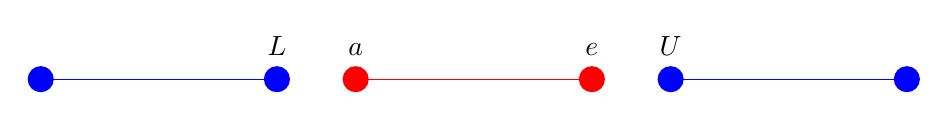
\begin{tikzpicture}[scale=2]
        \coordinate (A) at (0,0);
        \coordinate (B) at (1.5,0);
        \coordinate (C) at (2.0,0);
        \coordinate (D) at (3.5,0);
        \coordinate (E) at (4.0,0);
        \coordinate (F) at (5.5,0);

        \draw[blue] (A) -- (B);
        \draw[red]  (C) -- (D);
        \draw[blue] (E) -- (F);

        \node[circle,fill=blue,radius=0.15]                     at (A) {};
        \node[circle,fill=blue,radius=0.15,label=above : $L$]   at (B) {};
        \node[circle,fill=red,radius=0.15,label=above  : $a$] at (C) {};
        \node[circle,fill=red,radius=0.15,label=above  : $e$] at (D) {};
        \node[circle,fill=blue,radius=0.15,label=above : $U$]   at (E) {};
        \node[circle,fill=blue,radius=0.15]                     at (F) {};
    \end{tikzpicture}
\end{subfigure}

\par\bigskip

\begin{subfigure}{\textwidth}
    \centering
    \caption{Valid position: $L \leq u \leq d \leq e$}
    \label{subfig:all}
    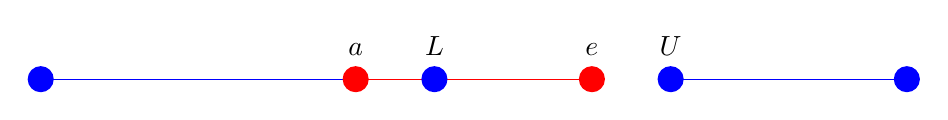
\begin{tikzpicture}[scale=2]
        \coordinate (A) at (0,0);
        \coordinate (B) at (2.5,0);
        \coordinate (C) at (2.0,0);
        \coordinate (D) at (3.5,0);
        \coordinate (E) at (4.0,0);
        \coordinate (F) at (5.5,0);

        \draw[blue] (A) -- (B);
        \draw[red]  (C) -- (D);
        \draw[blue] (E) -- (F);

        \node[circle,fill=blue,radius=0.15]                     at (A) {};
        \node[circle,fill=blue,radius=0.15,label=above : $L$]   at (B) {};
        \node[circle,fill=red,radius=0.15,label=above  : $a$] at (C) {};
        \node[circle,fill=red,radius=0.15,label=above  : $e$] at (D) {};
        \node[circle,fill=blue,radius=0.15,label=above : $U$]   at (E) {};
        \node[circle,fill=blue,radius=0.15]                     at (F) {};
    \end{tikzpicture}
\end{subfigure}

\par\bigskip

\begin{subfigure}{\textwidth}
    \centering
    \caption{Valid position: $a \leq u \le d \leq U$}
    \label{subfig:egu}
    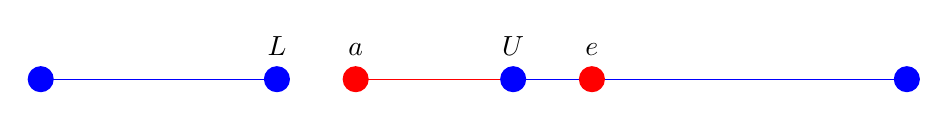
\begin{tikzpicture}[scale=2]
        \coordinate (A) at (0,0);
        \coordinate (B) at (1.5,0);
        \coordinate (C) at (2.0,0);
        \coordinate (D) at (3.5,0);
        \coordinate (E) at (3.0,0);
        \coordinate (F) at (5.5,0);

        \draw[blue] (A) -- (B);
        \draw[red]  (C) -- (D);
        \draw[blue] (E) -- (F);

        \node[circle,fill=blue,radius=0.15]                     at (A) {};
        \node[circle,fill=blue,radius=0.15,label=above : $L$]   at (B) {};
        \node[circle,fill=red,radius=0.15,label=above  : $a$] at (C) {};
        \node[circle,fill=red,radius=0.15,label=above  : $e$] at (D) {};
        \node[circle,fill=blue,radius=0.15,label=above : $U$]   at (E) {};
        \node[circle,fill=blue,radius=0.15]                     at (F) {};
    \end{tikzpicture}
\end{subfigure}

\par\bigskip

\begin{subfigure}{\textwidth}
    \centering
    \caption{Valid position: $L \le u \leq d \leq U$}
    \label{subfig:invertsandwhich}
    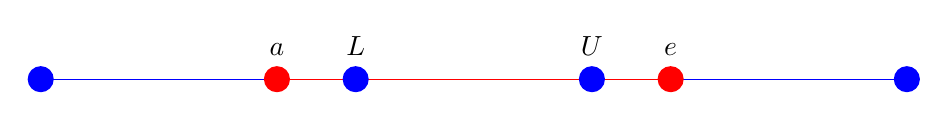
\begin{tikzpicture}[scale=2]
        \coordinate (A) at (0,0);
        \coordinate (B) at (1.5,0);
        \coordinate (C) at (2.0,0);
        \coordinate (D) at (3.5,0);
        \coordinate (E) at (4.0,0);
        \coordinate (F) at (5.5,0);

        \draw[blue] (A) -- (C);
        \draw[blue] (D) -- (F);
        \draw[red]  (B) -- (E);

        \node[circle,fill=blue,radius=0.15]                    at (A) {};
        \node[circle,fill=red,radius=0.15,label=above : $a$]   at (B) {};
        \node[circle,fill=blue,radius=0.15,label=above  : $L$] at (C) {};
        \node[circle,fill=blue,radius=0.15,label=above  : $U$] at (D) {};
        \node[circle,fill=red,radius=0.15,label=above : $e$]   at (E) {};
        \node[circle,fill=blue,radius=0.15]                    at (F) {};
    \end{tikzpicture}
\end{subfigure}

\par\bigskip

\begin{subfigure}{\textwidth}
    \centering
    \caption{Invalid position upper bound}
    \label{subfig:invalid-upper}
    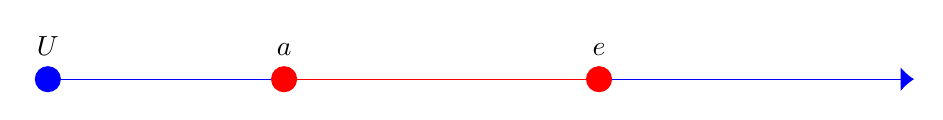
\begin{tikzpicture}[scale=2]
        \coordinate (A) at (0.0,0);
        \coordinate (B) at (5.5,0);
        \coordinate (C) at (1.5,0);
        \coordinate (D) at (3.5,0);

        \draw[-{Latex[width=3mm]},blue]  (A) -- (B);
        \draw[red]  (C) -- (D);

        \node[circle,fill=blue,radius=0.15,label=above : $U$] at (A) {};
        \node[circle,fill=red,radius=0.15,label=above  : $a$] at (C) {};
        \node[circle,fill=red,radius=0.15,label=above  : $e$] at (D) {};
    \end{tikzpicture}
\end{subfigure}

\par\bigskip

\begin{subfigure}{\textwidth}
    \centering
    \caption{Invalid position lower bound}
    \label{subfig:invalid-lower}
    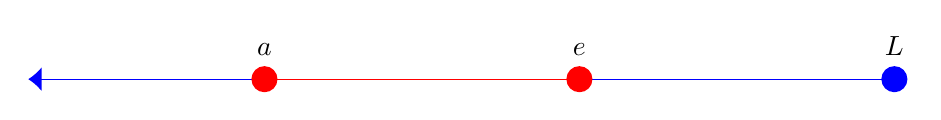
\begin{tikzpicture}[scale=2]
        \coordinate (A) at (0.0,0);
        \coordinate (B) at (5.5,0);
        \coordinate (C) at (1.5,0);
        \coordinate (D) at (3.5,0);

        \draw[-{Latex[width=3mm]},blue]  (B) -- (A);
        \draw[red]  (C) -- (D);

        \node[circle,fill=blue,radius=0.15,label=above : $L$] at (B) {};
        \node[circle,fill=red,radius=0.15,label=above  : $a$] at (C) {};
        \node[circle,fill=red,radius=0.15,label=above  : $e$] at (D) {};
    \end{tikzpicture}
\end{subfigure}

\caption{Outlines the different cases that requested time and charger allocated time can overlap}
\label{fig:find-free}
\end{figure}
\begin{algorithm}[H]
\caption{Find free time algorithm searches and returns the available time frames} \label{alg:find-free-time}
    \LinesNumbered
    \TitleOfAlgo{Find Free Time}
    \KwIn{$(C,a,e)$}
    \KwOut{($C',u,d)$}

    \tcc{Extract the lower and upper bounds.}
    L \(\leftarrow\) \(\{L \in C\}\)\;
    U \(\leftarrow\) \(\{L \in C\}\)\;

    \Begin
    {
        \If(\tcc*[f]{If $L < a < e < U]$ (\autoref{subfig:sandwich})}){$L \leq a$ and $U \geq e$}
        {
                u $\leftarrow$ $\U_{[a,e]}$\;
                d $\leftarrow$ $\U_{[u,e]}$\;
        }
        \ElseIf(\tcc*[f]{Else if $a < L < e < U$ (\autoref{subfig:all})}){$L > a$ and $U \geq e$}
        {
                u $\leftarrow$ $\U_{[L,e]}$\;
                d $\leftarrow$ $\U_{[u,e]}$\;
        }
        \ElseIf(\tcc*[f]{Else if $L < a < U < e$ (\autoref{subfig:egu})}){$L \leq a$ and $U < e$}
        {
                u $\leftarrow$ $\U_{[a,U]}$\;
                d $\leftarrow$ $\U_{[u,U]}$\;
        }
        \ElseIf(\tcc*[f]{Else if $a \leq u \leq d \leq L$ or $U \leq a \leq d \leq e$ (\autoref{subfig:invertsandwhich})}){$L > a$ and $U < e$}
        {
                u $\leftarrow$ $\U_{[a,L], [U,e]}$\;
                d $\leftarrow$ $\U_{[u,L], [u,e]}$\;
        }
        \Else(\tcc*[f]{Otherwise the bus cannot be scheduled in this time frame (\autoref{subfig:invalid-lower}, \autoref{subfig:invalid-upper})})
        {
                u $\leftarrow$ $\varnothing$\;
                d $\leftarrow$ $\varnothing$\;
        }

        \If (\tcc*[f]{If an assignment was made}) {$u,d \ne \varnothing$}
        {
            $C' \leftarrow C' \setminus [L,U]$\tcc*{Remove $[L,U]$ from the set of free time for the current charger}
            $C' \leftarrow \{[L,u], [d, U]\}$\tcc*{Update the charger free time slices}
        }

        \Return{($C',u,d$)}
    }
\end{algorithm}

\paragraph{Purge}
\label{sec:purge}
The purge primitive generator simply removes a visit from a charger schedule, \(\C\). This generator exists so that other
primitive generators may place the visit back into the schedule without creating duplicate entries in \(\C\). Line 2
updates \(\C\) with the set of visits excluding visit \(i\). Line 3 returns the updated set of charger availability.

\begin{algorithm}[H]
  \caption{Purge algorithm} \label{alg:purge}
    \LinesNumbered
    \TitleOfAlgo{Purge}
    \KwIn{$\Sol$}
    \KwOut{$\bar{\Sol}$}

    \Begin
    {
        $\bar{\C} \leftarrow \C \setminus \C_{v_i}^i$\tcc*{Remove assignment of visit $i$ to charger $v_i$}
        \Return{$\bar{\C}$}\tcc*{Return updated tuple}
    }
  \end{algorithm}

\paragraph{Slide visit}
\label{slide-visit}
Slide visit is used for buses that have already been scheduled. Because of the constraint \ref{seq:c10} there may be
some room to manipulate \(u_i\) and \(d_i\) within the window \([a_i, e_i]\). Two new values, \(u_i\) and \(d_i\) are randomly
selected with a uniform distribution that satisfy the constraint \(a_i \leq u_i \leq d_i \leq e_i\). Line 2 generates a new \([u_i,
d_i]\) utilizing the \texttt{findFreeTime} function. Line 3 applies and returns the updated visit.

\begin{algorithm}[H]
\caption{Slide Visit Algorithm} \label{alg:slide-visit}
    \LinesNumbered
    \TitleOfAlgo{Slide Visit}
    \KwIn{$\Sol$}
    \KwOut{$\bar{\Sol}$}

    \SetKwFunction{Purge}{Purge}

    \Begin
    {
      $\bar{\C} \leftarrow$\Purge{$\Sol$}\tcc*{Purge visit $i$ from charger availibility matrix}
      $C \leftarrow \bar{C}_{i.v_i}$\tcc*{Get the time availability of the visit just purged}

        \If(\tcc*[f]{If there is time available in $C$}){\findFreeTime{$C$, ($a_i, e_i$)} $\not\in \varnothing$}
        {
          \Return{($\I_{i.q},u,d,\bar{C}$)}\tcc*[f]{Return visit, note that $q$ is unchanged}
        }
        \Return{($\varnothing$)}\tcc*{Return nothing}
    }
  \end{algorithm}

\paragraph{New charger}
\label{new-charger}
The new charger generator (shown in \ref{alg:new-charger}) moves a visit \(\I_i\) to a new charging queue while
maintaining the same charge time, \([u_i, d_i]\). Line 2 loops through a randomly indexed set of charger queue indices.
Line 3 checks if there is an available time slice \([a_i, e_i]\) for charger \(q\). Line 4 sets the charge start/stop times
to the previous values. Line 5 sets and returns the updated visit.

\begin{algorithm}[H]
  \caption{New Charger Algorithm} \label{alg:new-charger} \LinesNumbered \TitleOfAlgo{New Charger} \KwIn{$\Sol$}
  \KwOut{$\bar{\Sol}$}

    \SetKwFunction{Purge}{Purge}

    \Begin
    {
      $\bar{\C} \leftarrow$\Purge{$\Sol$}\tcc*{Purge visit $i$ from charger availibility matrix}
      $q \leftarrow \mathcal{U}_{Q}$\tcc*{Select a random charging queue with a uniform distribution}

      \If(\tcc*[f]{If there is time available in $C_{q}$}){\findFreeTime{$C_{q}$, ($a_i, e_i$)} $\not\in \varnothing$}
      {
        \tcc{Return visit, note $u$ and $d$ are the original inital/final charge times.}
        \Return{($q,\I_{i.u}, \I_{i.d},\C$)}
      }

      \Return{($\varnothing$)}\tcc*{Return nothing}
    }
  \end{algorithm}

\paragraph{Wait}
\label{sec:wait}
The wait generator simply removes a bus from a charger queue and places it in its idle queue, \(v_i \in \{1,...,B\}\).

\begin{algorithm}[H]
\caption{Wait algorithm} \label{alg:wait}
    \LinesNumbered
    \TitleOfAlgo{Wait}
    \KwIn{$\Sol$}
    \KwOut{$\bar{\Sol}$}

    \SetKwFunction{Purge}{Purge}

    \Begin
    {
      $\bar{\C} \leftarrow$\Purge{$\Sol$}\tcc*{Purge visit $i$ from charger availibility matrix}
      \Return{$(\I_{i.b}, \I_{i.a}, \I_{i.e}, \bar{\C})$}\tcc*[f]{Return visit}
    }
  \end{algorithm}

\paragraph{New Window}
\label{sec:new-window}
New window is a combination of the wait and then new visit generators (\ref{sec:purge} and \ref{sec:new-visit}). By this it is
meant that current scheduled tuple \((v_i, u_i, d_i)\) is purged and added back in as if it were a new visit. Line 2
purges the BEB visit from the schedule and Line 3 places the BEB back into the schedule using the new visit generator.
Line 4 assigns and returns the updated visit.

\begin{algorithm}[H]
  \caption{New window algorithm} \label{alg:new-window}
  \LinesNumbered
  \TitleOfAlgo{New Window}
  \KwIn{$\Sol$}
  \KwOut{$\Sol'$}

  \SetKwFunction{NewVisit}{NewVisit}
  \SetKwFunction{Purge}{Purge}

  \Begin
  {
    $\bar{\C} \leftarrow$\Purge{$\Sol$}\tcc*{Purge visit $i$ from charger availibility matrix}
    \If(\tcc*[f]{Add visit $i$ back in randomly}) {($\bar{\I}, \bar{\C}) \leftarrow$ \NewVisit{$\Sol'$} $\not\in \Sol$}
    {
      \Return{($\bar{\I}, \bar{\C}$)} \tcc*[f]{Return visit}
    }

    \Return{($\varnothing$)}\tcc*{Return nothing}
  }
\end{algorithm}

\subsubsection{Generator Wrappers}
\label{sec:generator-wrappers}
This section covers the algorithms utilized to select and execute different generation processes for the SA process. The
generator wrappers are the methods immediately called by the SA algorithm. Each wrapper utilizes the generators
previously described and returns either a new charge schedule or a modified charge schedule.

\paragraph{Charge Schedule Generation}
\label{sec:charge-schedule-generation}
The objective of this generator is to generate a candidate solution provided a given route schedule. To generate a
candidate solution, the generator is given \(\I\), which represents the set of unscheduled BEBs. Line 3 loops through the
set of randomly indexed visits. Line 4 extracts the visit index and Line 5 generates a new visit and populates the
updated route information and charger schedule. This process is done for all visits \(i \in \Iset\).

\begin{algorithm}[H]
\caption{Charge schedule generation algorithm} \label{alg:charge-schedule-generation}
    \LinesNumbered
    \TitleOfAlgo{CSG}
    \KwIn{$\I$, $\C$}
    \KwOut{$\I'$, $\C'$}

    \SetKwFunction{NewVisit}{NewVisit}

    \Begin
    {
        $\I' \leftarrow \; \varnothing$\tcc*[f]{Begin with empty set of scheduled visits.}

        \tcc{Select an unscheduled BEB visit from a randomly indexed set of visits}
        \ForEach {$\I_i \in \{\ \U_{\I} \}$}
        {
            $i\leftarrow\; \I_i$\tcc*{Extract the visit index}
            ($\I'$, $\C'$) $\leftarrow$ \NewVisit{($i$, $\I$, $\C$)}\tcc*{Assign the bus to a charger}
        }
            \Return{($\I'$, $\C'$)}
    }
\end{algorithm}

\paragraph{Perturb Schedule}
\label{sec:tweak-schedule}
As described in SA, local searches are also employed to try and exploit a given solution
\cite{radosavljevic-2018-metah-optim}. After each step of the cooling function, the new candidate solution will be
altered by one primitive generation function and compared to the active solution. This process is done over many
iterations. That is, the local solution space shall be explored in an attempt to find an optima. The method that will be
employed to exploit the given solution is as follows: pick a visit, pick a primitive generator, and execute said
primitive generator. The algorithm is outlined in \ref{alg:perturb-schedule}. Line 2 selects a visit with a uniform
distribution. Let \(n_G\) denote the number of primitive generators available and let \texttt{PGF} be the primitive generation
function, Line 3 selects a primitive generation function with a uniform distribution. Line 5 executes the generation
function.

\begin{algorithm}[H]
\caption{Perturb schedule algorithm} \label{alg:perturb-schedule}

    \LinesNumbered
    \TitleOfAlgo{PS}
    \KwIn{$\I$, $\C$}
    \KwOut{$\I_i'$, $\C'$}

    \SetKwFunction{PGF}{PGF}

    \Begin
    {
        $\I_i\leftarrow\; \U_{\I}$\tcc*{Randomly select a visit}
        $i \leftarrow\; \I_i$\tcc*{Extract visit index}
        $PGF \leftarrow\; \U_{[1,n_G]}$\tcc*{Select one of the generator functions}
        $\Sol' \leftarrow$ \PGF{($i$, $\I$, $\C$)}\tcc*{Excecute the generator function}
        \Return{($\I'$, $\C'$)}
    }
\end{algorithm}
\section{Optimization Algorithm}
\label{sec:optimization-algorithm}
This section combines the generation algorithms and the optimization problem into a single algorithm. It begins with an
introduction and discussion of a general SA algorithm which will be used to springboard into the construction of the SA
PAP algorithm. For the case of the pseudo SA algorithm to be presented, the notation will be self-contained and not
related to any of the variables presented for SA PAP thus far.

\subsection{Simulated Annealing Pseudo Code}
\label{sec:simulated-annealing-pseudo-code}
Consider \ref{alg:sa-pseudo} \cite{henderson-1989-theor-pract}. Let \(\omega\) and \(\omega'\) are the current solution and the
candidate solution, respectively. Let \(\Tau\) denote the temperature function and \(\Tau_0\) the initial temperature.
Furthermore, let \(t\) be defined as the vector of temperatures defined by \(t = \Tau(\Tau_0, \Tau_f)\), and let \(t_k\) be
defined as being an element of \(t\), \(t_k \in t\). Let \(J\) be the repetition counter, it defines the number of iterations to
execute for each step in temperature, \(t_k\).

The algorithm behaves as follows: initialize the SA algorithm with an initial solution, temperature schedule, and
repetition schedule. The first loops through all the values in \(t_k\), the second loop finished when \(j = J\). For each
loop, create a new solution, \(N(\omega)\), calculate the difference in the fitness of \(\omega\) and \(\omega'\). Update \(\omega\) with \(\omega'\) if
the candidate solution is better or update \(\omega\) with \(\omega'\) with probability \(e^{\frac{-\Delta_{\omega , \omega'}}{t_k}}\) if the candidate
solution is worse than the current solution. Then the new candidate solution is modified slightly, \(M(\omega')\), to produce
an altered new candidate solution \(\omega{''}\). The modified candidate solution is then compared to \(\omega\) similarly as before.
The modifications then occurs over \(J\) iterations. This is repeated for all temperatures in \(t_k\).

\begin{algorithm}[H]
\caption{Pseudo-code for SA} \label{alg:sa-pseudo}
    \LinesNumbered
    \TitleOfAlgo{SA Pseudo-Code}

    \SetKwFunction{f}{f}
    \SetKwFunction{New}{N}
    \SetKwFunction{Mod}{M}
    \SetKwFunction{Temp}{$\Tau$}

    \Begin
    {
        $\omega \leftarrow$ New{($\I$, $\C$)}\tcc*{Generate an initial solution}

        \tcc{Generate vector of temperatures given temperature function $\Tau$ and initial temperature $\Tau_0$}
        $t \leftarrow$ \Temp{$\Tau_0$}

        \ForEach{$t_k \in t$}
        {
            $j \leftarrow 0$ \tcc*{Set repetition counter}
            $\omega' \leftarrow $ \New{($\I$, $\C$)} \tcc*{Generate a new solution}
            $\Delta_{\omega,\omega'} \rightarrow$ \f{$\omega'$} - \f{$\omega$} \tcc*{Calculate the difference of fitness scores}
            \If{$\Delta_{\omega , \omega'} \le 0$}{$\omega \rightarrow \omega'$}
            \If{$\Delta_{\omega , \omega'} > 0$}{$\omega \rightarrow \omega'$ with probability $e^{\frac{-\Delta_{\omega , \omega'}}{t_k}}$}

            \While{$j \le J$}
            {
                $\omega{''} \leftarrow$ \Mod{($\I'$, $\C'$)} \tcc*{Modify the new solution}
                $\Delta_{\omega,\omega{''}} \rightarrow$ \f{$\omega{''}$} - \f{$\omega$} \tcc*{Calculate the difference of fitness scores}
                \If{$\Delta_{\omega , \omega{''}} \le 0$}{$\omega \rightarrow \omega{''}$}
                \If{$\Delta_{\omega , \omega{''}} > 0$}{$\omega \rightarrow \omega{''}$ with probability $e^{\frac{-\Delta_{\omega , \omega{''}}}{t_k}}$}
                $j \leftarrow j+1$\;
            }
        }
    }
\end{algorithm}

\subsection{SA PAP Pseudo Code}
\label{sec:sa-pap-pseudo-code}
Now that the general SA algorithm has been outlined, the objective is now to outline SA-PAP in \ref{alg:sa-pap}. While
the SA PAP generally is outlined almost identically to that of the general SA algorithm, SA assumes that the new
solution generated, \(\omega'\) in the case of \ref{alg:sa-pseudo}, is in the solution space of the problem, \(\omega \in S\) where \(S\)
is the solution space. Referring to \ref{alg:charge-schedule-generation}, the generating function for SA PAP, note that
assignments are made at random. One is to expect that the output generated by this function may not be in the solution
space. Therefore, the constraints introduced in \ref{sec:constraints} must be employed to verify that the output of
\ref{alg:charge-schedule-generation} is in the feasible space.

As previously stated, the generating functions directly influence the values of the assigned charge queue, charge
initialization time, and charge completion time: \(v_i\), \(u_i\), and \(d_i\), respectively. Having generated those values,
the rest of the decision variables may be derived. Let's begin by reviewing over the packing constraints.
\ref{seq:c0}-\ref{seq:c1} are employed to enable and disable \(\sigma_{ij}\) and \(\psi_{ij}\) and \ref{seq:c2}-\ref{seq:c4} ensure
the validity of the set values. \ref{seq:c5} can be directly calculated and \ref{seq:c11} is fully defined.

Now let's change the focus over to the dynamic constraints. Similar to what was seen with the packing constraints, the
battery dynamic constraints are also fully defined and can be calculated. \ref{seq:c6} is sequentially calculated while
\ref{seq:c7}-\ref{seq:c9} can be evaluated to ensure the charge propagation is feasible. Thus, the constraints to
enable/disable the penalty function, \ref{seq:c9}-\ref{seq:c10}, can be executed to determine the value of \(\phi_i\) for
each visit. \ref{seq:c12}-\ref{seq:c15} may also be evaluated to find the values of \(\theta_h^{v_i}\) and \(\mu_h^{v_i}\) which
then directly leads to \ref{seq:c16} being able to be determined. Once all these constraints have been calculated and
evaluated to be true will a generated solution be considered in the feasible space. Let the feasible space be denoted as
\(S\).

Lines 2-3 initialize the SA algorithm by creating a vector of temperature values based on a temperature schedule \(\Tau\),
and an initial temperature \(\Tau_0\) and then generating an initial solution. Line 4 loops through each of the step in
the temperature schedule \(t_k \in t\). Lines 4 and 5 generates a new solution then calculates its fitness. \(\nu\) in this
context is defined as \(\nu = (u, d, v, \eta)\). Lines 6 through 11 update the solution depending on if the new solution is in
the solution space a whether the new solution is more or less fit than the active solution. Line 12 iterates through the
repetition schedule, \(k \in \{1, 2, ..., n_K\}\). Lines 13 perturbs the previously generated solution. Lines 15-20
calculates its fitness, and updates the current solution with the candidate solution depends upon whether the newly
generated solution is in the solution space and also the fitness in the same was that was done before.

\begin{algorithm}[H]
\caption{Simulated annealing approach to the position allocation problem} \label{alg:sa-pap}
    \LinesNumbered
    \TitleOfAlgo{SA PAP}
    \KwIn{($\I$ , $\C$)}
    \KwOut{($\I'$, $\C'$)}

    \SetKwFunction{Temp}{$\Tau$}
    \SetKwFunction{CSG}{CSG}
    \SetKwFunction{PS}{PS}
    \SetKwFunction{Obj}{J}

    \Begin
    {
        \tcc{Generate vector of temperatures given temperature function $\Tau$ and initial temperature $\Tau_0$}
        $t \leftarrow$ \Temp{$\Tau_0$}

        $\nu \leftarrow$\CSG{($\I$, $\C$)}\tcc{Generate an initial solution}

        \tcc{For each item in the temperature vector}
        \ForEach{$t_k \in t$}
        {
            $\upsilon' \subset (\I', \C') \leftarrow$ \CSG{($\I$, $\C$)} \tcc*{Generate a new solution}
            $\Nu_{\upsilon, \upsilon'} = $ \Obj{$\upsilon'$}  - \Obj{$\upsilon$} \tcc*{Calculate the difference of fitness scores}

            \If{$\I' \in S$ and $\Nu_{\upsilon, \upsilon'} \le 0$}{$\upsilon \leftarrow \upsilon'$}
            \If{$\I' \in S$ and $\Nu_{\upsilon, \upsilon'} \ge 0$}{$\upsilon \leftarrow \upsilon'$ with probability $e^{\frac{\Nu_{\upsilon, \upsilon'}}{t_k}}$}

            \tcc{For each step in the repitition schedule} \ForEach{$k \in \{1, 2, ..., n_K\}$} { $\upsilon{''} \subset
              (\I', \C') \leftarrow$ \PS{($\I'$, $\C'$)} \tcc*{Perturb the solution} $\Nu_{\upsilon, \upsilon{''}} = $
              \Obj{$\upsilon{''}$} - \Obj{$\upsilon$} \tcc*{Calculate the difference of fitness scores}

                \If{$\I' \in S$ and $\Nu_{\upsilon, \upsilon{''}} \le 0$}{$\upsilon \leftarrow \upsilon{''}$}
                \If{$\I' \in S$ and $\Nu_{\upsilon, \upsilon{''}} \ge 0$}{$\upsilon \leftarrow \upsilon{''}$ with probability $e^{\frac{\Nu_{\upsilon, \upsilon{''}}}{t_k}}$}
            } % For k
        }     % For t_k \in t

        \Return{($\I'$ , $\C'$)} } % Begin
\end{algorithm}


\bibliographystyle{plain}
\bibliography{/home/alex/Documents/citation-database/lit-ref,/home/alex/Documents/citation-database/lib-ref}
\end{document}